\begin{surferPage}[216-singularit\u{a}\c{t}i]{Suprafe\c{t}e cu multe singularit\u{a}\c{t}i reale}
   A\c{s}a cum am mai men\c{t}ionat, num\u{a}rul maxim posibil $\mu(7)$ de singularit\u{a}\c{t}i pe o suprafa\c{t}\u{a} de grad $7$ nu este
    cunoscut cu exactitate. Avem doar o limit\u{a} superioar\u{a} \c{s}i inferioar\u{a}: $99 \le \mu(7) \le 104$.

    Astfel, nu este foarte surprinz\u{a}tor faptul c\u{a} \c{s}i mai pu\c{t}in este cunoscut pentru un grad general $d$.
    
    Cu toate acestea, Sonja Breske, Oliver Labs \c{s}i Duco van Straten au reu\c{s}it s\u{a} adapteze o
    construc\c{t}ie a lui S.V. \ Chmutov, astfel \^{i}nc\^{a}t numarul maxim actual de singularit\u{a}\c{t}i este atins \c{s}i de suprafe\c{t}e cu singularit\u{a}\c{t}i 
    reale.
    P\^{a}n\u{a} acum \c{s}tim:
    \[0,41\bar{6}d^3 \lessapprox \mu(d) \lessapprox 0.44\bar{4} d^3.\]
    De mai sus, se poate observa simetria construc\c{t}iei \c{s}i o rela\c{t}ie cu num\u{a}rul maxim de celule negre \^{i}ntr-un aranjament de drepte:
    \begin{center}
      \begin{tabular}{c@{\qquad}c}
        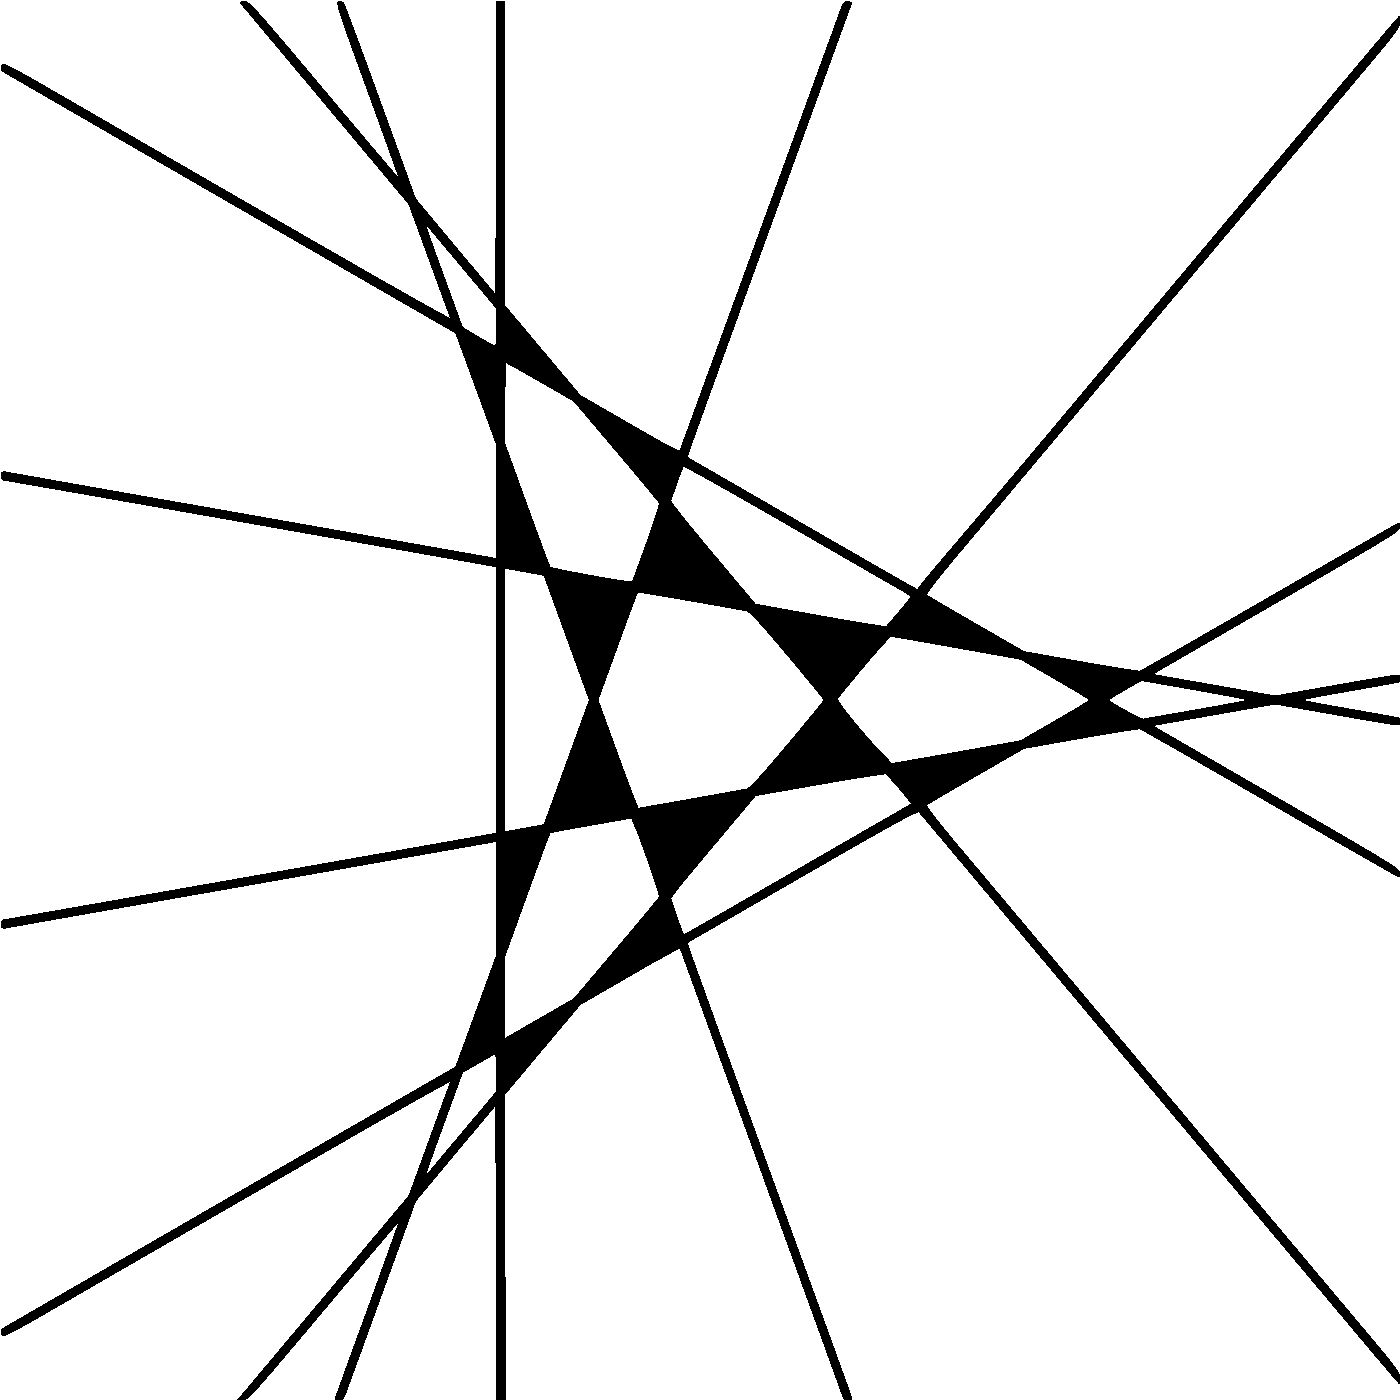
\includegraphics[height=1.5cm]{./../../common/images/vielesing.pdf}
        &
        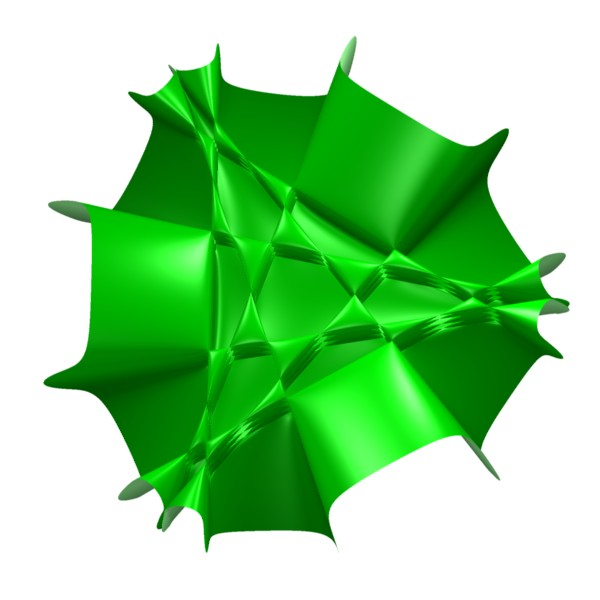
\includegraphics[height=1.5cm]{./../../common/images/p9surface_von_oben}
      \end{tabular}
    \end{center}
\end{surferPage}
